\chapter{Herramientas empleadas para la realización del proyecto}

\section{Introducción}
Habiendo tratado en el capítulo anterior el fundamento teórico que concierne a las nubes de puntos y el procesamiento software de las mismas se procede en este capítulo a explicar con mayor profundidad las herramientas necesarias para cumplir los objetivos propuestos para el presente trabajo.



\section{Descripción de herramientas para desarrollar el trabajo}
Para realizar el presente trabajo se requieren herramientas que pueden clasificarse en dos tipos: software y hardware.

\subsection{Herramientas software}
\subsubsection{Máquina virtual}
Se hace uso de una máquina virtual con Ubuntu\cite{ubuntu} 18.04.1 64 bits ya que es un sistema operativo que facilita la instalación y uso de PCL y otras librerías, no como Windows.
Por lo tanto, a partir de este punto, salvo que se mencione lo contrario, el sistema de archivos e instrucciones ejecutadas por línea de comandos así como demás características propias de diferentes sistemas operativos se refieren a un sistema operativo basado en Linux.
\\
\\
La máquina virtual se crea haciendo uso del software VirtualBox\cite{virtualbox} el cual facilita la creación y personalización de máquinas virtuales no solamente basadas en Linux sino con cualquier otro sistema operativo.

%https://www.virtualbox.org/
\subsubsection{Instalación de PCL sobre un sistema basado en Linux}
Una vez se dispone de la máquina virtual, es necesario instalar las librerías de PCL\cite{pcl_installation}. Para ello se visita la web oficial de PCL pues ésta ofrece las instrucciones adecuadas. Para poder instalar PCL en linux se deben ejecutar los siguientes comandos:

%http://pointclouds.org/downloads/

\begin{verbatim}
sudo add-apt-repository ppa:v-launchpad-jochen-sprickerhof-de/pcl
sudo apt-get update
sudo apt-get install libpcl-all
\end{verbatim}

La primera instrucción añade al sistema el repositorio en el que se encuentra la librería, el segundo busca actualizaciones disponibles y por último se procede a la instalación de todos los archivos actualizados.
\\
\\
Estas mismas instrucciones sirven para instalar PCL en el sistema embebido ya que dispone del un sistema operativo Debian basado en Linux.
\\
\\
Cuando la instalación está completa, se generan una serie de carpetas en el directorio /usr/include:

\begin{itemize}
\item[•]pcl-1.8: Es la versión 1.8 de la librería de PCL. Contiene en su interior la carpeta pcl que con todos los módulos de PCL estructurados correctamente.
\item[•]eigen3: Librería eigen que se encuentra bajo la carpeta Eigen dentro de este directorio.
\item[•]FLANN: Librería FLANN que se encuentra bajo la carpeta flann dentro de este directorio.
\item[•]vtk-x: versión x de la librería vtk 
\end{itemize}

\subsubsection{Vivado Design Suite HLx Editions}
Ya está instalado PCL en el sistema, ahora falta adquirir una herramienta para síntesis de alto nivel.
\\
\\
La síntesis de alto nivel, del inglés High Level Synthesis (HLS) es un proceso de diseño automático que interpreta una descripción algorítmica en software de un comportamiento deseado y crea hardware digital que lo implementa.
\\
\\
La síntesis comienza con una descripción en alto nivel del problema o comportamiento que desea reproducirse. Para ello se puede utilizar uno de los varios lenguajes de programación en alto nivel como C o C++. Este código es entonces analizado y programado para ser compilado en lo que se conoce como un Register Transfer Level (RTL), es decir, la abstracción del diseño que modela un circuito digital síncrono en sus señales entre registros y las operaciones realizadas sobre ellas.  El diseño de hardware puede ser generado a diferentes niveles de abstracción: puertas lógicas, registros y algoritmos. Se aprecia en la figura \ref{fig:circuito} un diseño hardware a nivel de registro de un circuito inversor.
\begin{figure}[!htb]
\centering
\includegraphics[scale=0.25]{circuito}
  \caption{Circuito digital síncrono que actúa como un inversor de la señal de entrada.}\label{fig:circuito}
\end{figure}

El RTL queda definido mediante un Hardware Description Language (HDL) del inglés, lenguaje de descripción de hardware como VHDL o Verilog. Para el caso del ejemplo anterior y tomando VHDL como el lenguaje de descripción, la definición del circuito de la figura \ref{fig:circuito} queda como:

\begin{lstlisting}[language=VHDL,breaklines]
D <= not Q;
 
process(clk)
begin
    if rising_edge(clk) then
        Q <= D;
    end if;
end process;
\end{lstlisting}


El objetivo de la síntesis en alto nivel es permitir a los diseñadores construir y verificar hardware de forma eficiente así como el de dotarles de mayor control y optimización sobre sus diseños con la facilidad añadida de poder definirlos mediante lenguajes de alto nivel de abstracción mientras la herramienta realiza la implementación del RTL de forma automática.
\\
\\
Para realizar la síntesis de alto nivel se elige la herramienta vivado HLS de Xilinx. Accediendo a la web oficial de descargas\cite{vivado_descarga} se puede descargar la versión deseada de este software ya sea como un archivo comprimido un instalador web para mayor comodidad. En este caso se elige la versión 2017.1
\\
\\
Haciendo uso del mencionado software de Xilinx, se define en un lenguaje de programación de alto nivel, por ejemplo C++, un comportamiento que se implementa como una función con sus argumentos, operaciones internas y un valor de retorno. Además, deben definirse unos ``pragmas'', es decir, una región de código considerada como un protocolo y en el que Vivado HLS no introduce ninguna señal de reloj excepto si se indica explícitamente. Una región definida como un protocolo puede ser utilizada para especificar de forma manual una interfaz de conexión a otros bloques hardware con el mismo protocolo de entrada/salida de señales. Esto implica que, por ejemplo, dado un bloque hardware, se pueden definir dos buses: un bus IN que contiene todas las señales de entrada al bloque y un bus OUT que contiene todas las señales salientes.


%https://www.xilinx.com/support/download.html
%https://www.xilinx.com/products/design-tools/vivado/integration/esl-design.html

\subsection{Herramientas hardware} \label{herraminetas_hardware}
La principal herramienta hardware de la que se dispone y sobre la cual se comprobarán los resultados de la aplicación de los objetivos del presente trabajo es la placa de desarrollo Pynq-Z1\cite{pynq} que se puede ver en la figura \ref{fig:pynq}. Se trata de una placa de bajo coste y ampliamente utilizada en universidades y centros de investigación.

\begin{figure}[H]
\centering
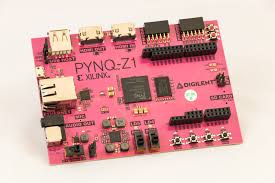
\includegraphics[scale=1.0]{pynq}
  \caption{Placa de desarrollo Pynq-Z1 de Xilinx.}\label{fig:pynq}
\end{figure}

Esta placa dispone de un System on Programmable Chip (SoPC) del inglés sistema en chip programable, del modelo Zynq xc7z020clg400-1. Un sistema en chip programable es la combinación de núcleos de procesamiento de una CPU (Central Processing Unit o unidad central de procesamiento) con hardware personalizado que se implementa normalmente con una FPGA y bloques de memoria.
\\
\\
Una FPGA, siglas del inglés ``Field Programmable Gate Array'' o matriz de puertas programables es un dispositivo programable que contiene bloques de lógica cuya interconexión y funcionalidad pueden ser reconfiguradas en tiempo de ejecución.
\\
Además, una FPGA dispone de dos capas: aplicación y configuración. La primera se compone de todos sus recursos hardware que han de ser configurados e interconectados haciendo uso de la segunda, la capa de configuración en la que se carga un ``bitstream'' es decir un archivo de configuración que se puede generar, entre otras formas, haciendo uso del programa Vivado de Xilinx y que permite para cada ``bitstream'' que se cargue, dotar a la FPGA de diferentes funcionalidades.
\\
\\
Volviendo al ámbito de un SoPC, los núcleos del procesador pueden ser ``hard'' (duros) o ``soft'' (blandos): los primeros son permanentemente embebidos en silicio mientras que los segundos se implementan usando recursos de una FPGA. 
\\
Los núcleos duros ofrecen mucho rendimiento y bajo consumo pero son poco flexibles en cuanto a las operaciones que pueden realizar. Éstos forman el Processing System (PS) dentro del SoPC para rutinas software y operaciones relacionadas con sistemas operativos a diferencia de la FPGA que conforma la Programmable Logic (PL) que sirve para implementar lógica de alta velocidad y aritmética.
\\
La PS dispone en este caso de un sistema operativo Debian basado en el kernel Linux.
\\
\\
%http://ati.ttu.ee/~alsu/05_SoPC.pdf
Algunas de las características principales del PS del SoPC mencionado son:

\begin{itemize}
\item[•] Un procesador Cortex-A9 de dos núcleos a 650MHz y arquitectura ARM, memoria caché de nivel 1 con 32KB pra instrucciones y 32KB para datos, memoria caché de nivel 2 y 512KB y memoria en chip de 256KB.
\item[•] Controlador de memoria DDR3 con 8 canales DMA y 4 puertos esclavos AXI3 de alto rendimiento
\item[•] Controladores de periféricos con elevado ancho de banda: Ethernet 1G, USB 2.0 y SDIO 
\item[•] Controlador de periféricos de gran ancho de banda: SPI, UART, CAN, I2C
\item[•] 630KB de memoria RAM
\item[•] Programable con JTAG, flash Quad-SPI y tarjeta micro SD
\end{itemize}


En cuanto al PL del SoPC:
\begin{itemize}
\item[•] 13300 secciones de lógica cada una de ellas con 4 Look-up Tables de 6 entradas y 8 Flip-Flops
\item[•]630KB de block RAM
\item[•] 4 unidades de administración de la señal de reloj
\item[•] 220 secciones de lógica para procesamiento de señales digitales (DSP)
\item[•] Conversor analógico-digital integrado en chip (XADC)

\end{itemize}

\section{Conclusiones}
Con el cierre del presente capítulo terminan las explicaciones fundamentales tanto de teoría como de herramientas que permiten estructurar el TFG.
\\
En el siguiente capítulo se mostrarán las primeras tareas que giran entorno a la librería PCL para así poder visualizar nubes de puntos y extraer keypoints de las mismas.

